% Figure: Trigger-Capable Mechanism Relationships
% Diamond layout showing interconnections among the 4 root cause mechanisms

\begin{figure}[htbp]
\centering
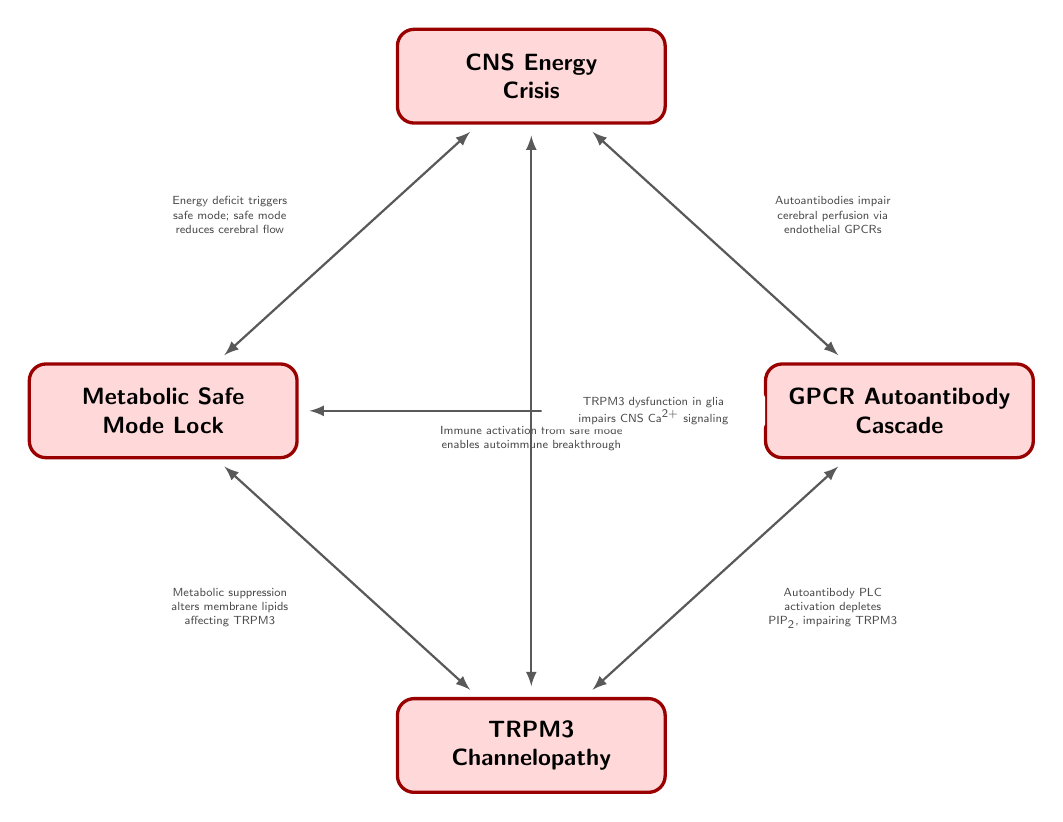
\begin{tikzpicture}[
    scale=0.85, every node/.style={scale=0.85, font=\sffamily},
    % Root cause node style
    root cause/.style={
        rectangle, rounded corners=6pt,
        draw=red!60!black, fill=red!15, very thick,
        minimum width=4cm, minimum height=1.4cm,
        font=\sffamily\bfseries, align=center,
        inner sep=6pt
    },
    % Bidirectional edge style
    interaction/.style={
        <->, >=latex, thick, gray!70!black,
        shorten >=4pt, shorten <=4pt
    },
    % Edge label style
    edge label/.style={
        font=\sffamily\tiny, fill=white, inner sep=2pt,
        text=gray!60!black, align=center, rounded corners=2pt,
        text width=3.2cm
    }
]

% --- Nodes in diamond layout ---
% Top
\node[root cause] (cns) at (0, 5) {CNS Energy\\Crisis};
% Left
\node[root cause] (safe) at (-5.5, 0) {Metabolic Safe\\Mode Lock};
% Right
\node[root cause] (gpcr) at (5.5, 0) {GPCR Autoantibody\\Cascade};
% Bottom
\node[root cause] (trpm) at (0, -5) {TRPM3\\Channelopathy};

% --- Edges with labels ---

% CNS <-> Safe Mode (top-left diagonal)
\draw[interaction] (cns) -- (safe)
    node[edge label, pos=0.5, above left=2pt] {Energy deficit triggers\\safe mode; safe mode\\reduces cerebral flow};

% CNS <-> GPCR (top-right diagonal)
\draw[interaction] (cns) -- (gpcr)
    node[edge label, pos=0.5, above right=2pt] {Autoantibodies impair\\cerebral perfusion via\\endothelial GPCRs};

% Safe Mode <-> TRPM3 (bottom-left diagonal)
\draw[interaction] (safe) -- (trpm)
    node[edge label, pos=0.5, below left=2pt] {Metabolic suppression\\alters membrane lipids\\affecting TRPM3};

% GPCR <-> TRPM3 (bottom-right diagonal)
\draw[interaction] (gpcr) -- (trpm)
    node[edge label, pos=0.5, below right=2pt] {Autoantibody PLC\\activation depletes\\PIP\textsubscript{2}, impairing TRPM3};

% Safe Mode <-> GPCR (horizontal, bottom middle)
\draw[interaction] (safe) -- (gpcr)
    node[edge label, pos=0.5, below=4pt] {Immune activation from safe mode\\enables autoimmune breakthrough};

% CNS <-> TRPM3 (vertical, through center)
\draw[interaction] (cns) -- (trpm)
    node[edge label, pos=0.5, right=4pt] {TRPM3 dysfunction in glia\\impairs CNS Ca\textsuperscript{2+} signaling};

\end{tikzpicture}
\caption{Interconnections among trigger-capable root cause mechanisms.
All four mechanisms can co-activate and reinforce each other, complicating
the identification of the initiating cause in individual patients
(Section~\ref{sec:root-cause-relationships}).}
\label{fig:trigger-relationships}
\end{figure}
